\subsection{Informationsquellen im Web}\label{subsec:Informationsquellen}
In Bezug auf Web-Feeds spricht man von \glqq{}Content Syndication\grqq{}, was im deutschsprachigen Raum als \glqq{}Syndikation\grqq{} bezeichnet wird. Eine m�gliche Spezifikation definiert Syndikation als Bereitstellung von Daten f�r weitere �bertragung, Aggregierung und Online-Publikation\footnote{http://web.resource.org/rss/1.0/}. Ein verbreitetes Format f�r Web-Feeds stellt RSS dar.\\
Je nach Quelle wird die Abk�rzung RSS unterschiedlich interpretiert. In der ersten Version (RSS 1.0) stand die Abk�rzung f�r \glqq{}RDF Site Summary\grqq{}. In der Version 2.0 wird jedoch \glqq{}Really Simple Syndikation\grqq{}\footnote{https://validator.w3.org/feed/docs/rss2.html\label{rss2.0}} erw�hnt. Allgemein stellt RSS ein XML-basiertes Format dar, das urspr�nglich besondere Verbreitung im Bereich von Webblogs gefunden hat \cite[S.103]{tilkov2015}. Im Laufe der Zeit hat sich RSS allgemein als gut funktionierendes Mittel zur Benachrichtigung von �nderungen erwiesen, obwohl es laut Tilkov et al. \cite{tilkov2015} kein Standard von hoher Qualit�t sei.\\
Die Definition eines Eintrages in RSS 2.0 Format erfolgt im Rss-Tag, der den Namensraum der verwendeten Elemente und die Version von RSS umfasst. Im Rss-Tag wird der Channel-Tag definiert, der die Daten beschreibt. Im Channel-Tag m�ssen folgende Elemente vorhanden sein (siehe \ref{rss2.0}):
\begin{itemize}
\item Title: Name des Kanals (Channel)
\item Link: URL zur Webseite des entsprechenden Kanals
\item Description: kurze Zusammenfassung des Kanals
\end{itemize} 
Die Inhalte des Channels werden durch als Items dargestellt. Laut der Spezifikation in \ref{rss2.0} entspricht ein Item einer Story. Man kann sich eine Story als ein Eintrag in der Zeitung vorstellen. Ein Item enth�lt keine Pflichtfelder. Allerdings muss entweder Title oder Description vorhanden sein. Ein Beispiel eines RSS-Eintrags von Heroku News-Feed\footnote{https://blog.heroku.com/news/feed} wird in Listing \ref{rss} dargestellt.
\begin{lstlisting}[basicstyle=\ttfamily, breaklines=true, label=rss,
					captionpos=b, caption={Beispiel eines Eintrages in RSS 2.0}]
<rss xmlns:dc="http://purl.org/dc/elements/1.1/" version="2.0">
 <channel>
  <title>Heroku</title>
  <link>http://blog.heroku.com</link>
  <description>The Heroku Blog</description>
  <item>
   <title>The Heroku-16 Stack is Now Available</title>
   <link>https://blog.heroku.com/heroku-16-is-generally-available</link>
   <pubDate>Thu, 20 Apr 2017 15:06:00 GMT</pubDate>
   <guid>https://blog.heroku.com/heroku-16-is-generally-available</guid>
   <description>
    <p>Your Heroku applications run on top of ...</p> 
   </description>
   <author>Jon Byrum</author>
  </item>
 </channel>
</rss>
\end{lstlisting}
Im Beispiel von Heroku werden au�erdem separate Feed-Channels f�r die unterschiedlichen Themenbereiche angeboten, wie es in Abbildung \ref{fig:heroku-feeds} zu sehen ist.
\begin{figure}[H] 
	\centering
	
\includegraphics[width=1.0\textwidth]{images/heroku-feeds.png}
	\caption{Feed-Channels von Heroku}
	\label{fig:heroku-feeds}
\end{figure}
Der Themenbereich umfasst sowohl allgemeine (z.B. Heroku Blog) als auch spezifische Informationen (z.B. Dev Center Articles). Im Anwendungsfall von \textit{PaaSfinder} ist der Dev Center Changelog Channel besonders relevant, da der die �nderungen im Bereich Entwicklung erl�utert (siehe Abbildung \ref{fig:heroku-changelog-feed}).
\begin{figure}[H] 
	\centering
	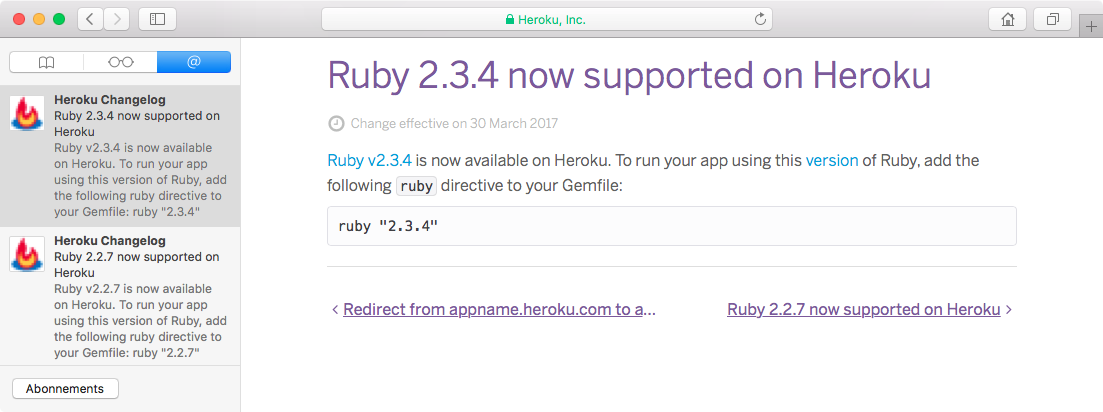
\includegraphics[width=1.0\textwidth]{images/heroku-changelog.png}
	\caption{Heroku Feed}
	\label{fig:heroku-changelog-feed}
\end{figure}
Der einfachste Weg zum Beziehen von Feeds stellt der Browser dar. Durch die Einbindung der Feed-Adressen wird bereits die Arbeit der regelm��igen Seitenaufrufs abgenommen. Allerdings sollen die Feeds immer noch maschinell analysiert werden. Eine m�gliche Automatisierung w�re der Ansatz eines RSS-Clients, der die Inhalte nach bestimmten Schl�sselw�rtern (z.B. Ruby) durchsucht. \\
Eine weitere Quelle der Updates sind soziale Plattformen wie Twitter oder Facebook. Beispiel